\chapter{More on slope}
%\addcontentsline{toc}{chapter}{1 Graphs}
%%%%%%%%%%%%%%% SECTION HEADER %%%%%%%%%%%%%%%%
\rhead{4}
\lhead{More on slope}
%%%%%%%%%%%%%%%%%%% START %%%$%%%%%%%%%%%%%%%%%
\section{Parallel lines}
When you graph two or more linear equations in a coordinate plane, they generally cross at a point. However, when two lines in a coordinate plane never cross, they are called parallel lines. 	\textbf{When two lines are parallel, their slopes are equal to each other.}
\begin{tcolorbox}[
                    title=Parallel lines,
                    fonttitle=\bfseries
                    colframe=blue!70!red,
                    colback=white
                    ]
	Let's consider two parallel lines. If the slope of first line is $m_1$ and the slope of other line is $m_2$, then 
    	\begin{equation}
    		m_1=m_2	\label{parallel}
    	\end{equation}
    \begin{center}
    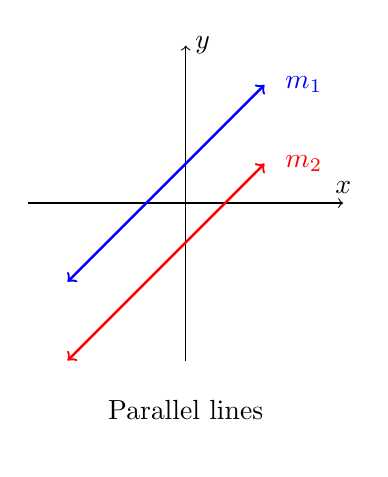
\begin{tikzpicture}
		\draw[->] (-2,0) -- (2,0) node[pos=1, above] {$x$};
		\draw[->] (0,-2) -- (0,2) node[pos=1, right] {$y$};
    	\draw[<->,line width=0.3mm, red] (-1.5,-2) -- (1,0.5);
        \node[text=blue] at (1.5,1.5) {$m_1$};
    	\draw[<->,line width=0.3mm, blue] (-1.5,-1) -- (1,1.5);
        \node[text=red] at (1.5,0.5) {$m_2$};
    	\node[label={Parallel lines}] at (0,-3) {};
	\end{tikzpicture}
    \end{center}
\end{tcolorbox}
% ========== Example 1
\begin{exa}
	Write an equation of line passing through $(-2,\,5)$ and parallel to the line whose equation is $y=3x-1$. Express the equation in slope-intercept form.
\end{exa}

To find the equation of a line, we need its slope and one point on the line. The point on the line is given $(-2,\,5)$.\\
Since the line is parallel to $y=3x-1$, then their slopes are equal to each other. The slope of $y=3x-1$ is 3, thus the slope of our line is also $m=3$. Using the point-slope formula:
\begin{align*}
        y-y_1=m(x-x_1)& &   &\text{Substitute slope and given point}\\
        y-(5)=2(x-(-2)& &   &\text{Simplify}\\
        y-5 = 2(x+2)&   &   &\text{Distribute 2 on LHS}\\
        y -5 = 2x+4&    &   &\text{Add 5 to both sides}\\
        y = 2x+9&   &   &\text{Our answer in slope-intercept form}
\end{align*}
% ============
\section{Perpendicular lines}
We also might have a case where two lines in the coordinate plane cross at a right angle. These are called perpendicular lines. \textbf{In this case, the slope of one line is negative reciprocal of slope of the other line.}
\begin{tcolorbox}[
                        title=Perpendicular lines,
                        fonttitle=\bfseries,
                        colframe=blue!70!red,
                        colback=white
                        ]
	Consider two perpendicular lines with slope of $m_1$ and $m_2$. The relationship between their slope is
    	\begin{equation}
    		m_1\,m_2=-1 \label{perpendicular}
    	\end{equation}
    \begin{center}
    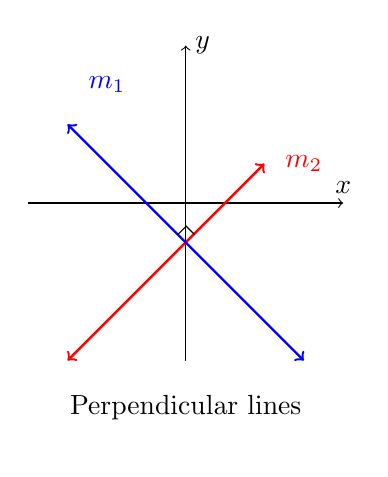
\begin{tikzpicture}
		\draw[->] (-2,0) -- (2,0) node[pos=1, above] {$x$};
		\draw[->] (0,-2) -- (0,2) node[pos=1, right] {$y$};
    	\draw[<->,line width=0.3mm, red] (-1.5,-2) -- (1,0.5);
        \node[text=blue] at (-1,1.5) {$m_1$};
    	\draw[<->,line width=0.3mm, blue] (-1.5,1) -- (1.5,-2);
        \node[text=red] at (1.5,0.5) {$m_2$};
    	\node[label={Perpendicular lines}] at (0,-3) {};
        \draw [rotate around={-45:(-0.1,-0.4)}] 
        				(-0.1,-0.4) -- ++(0,0.15) -- ++(0.15,0);
	\end{tikzpicture}
    \end{center}
\end{tcolorbox}
% ========== Example 2
\begin{exa} \leavevmode 
    \begin{enumerate}[a., font=\bfseries]
        \item Find the slope of any line that is perpendicular to the line whose equation is $x+3y-12=0$.
        \item Write the equation of line passing through $(-2,\,-6)$ and perpendicular to the line whose equation is $x+3y-12=0$. Express the equation in general form.
    \end{enumerate}
\end{exa}

\newpage
a. Let' call the given line $x+y-12=0$, $l_1$ and the line we are looking for $l_2$. We begin by converting $l_1$ into slope-intercept form
\begin{align*}
    l_1: x+3y-12=0&  &   &\text{Isolate $y$, subtract $x$}\\
    3y -12 = -x&    &   &\text{Add 12}\\
    2y = -x+12& &   &\text{Divide by 2}\\
    y = -\frac{1}{2}x+6&    &   &\text{Slope-intercept form}
\end{align*}
The slope of $l_1$ is $-1/2$. Since $l_2$ is perpendicular to $l_1$, the slope of $l_2$ will be
\begin{align*}
    m_2= -\frac{1}{m_1}&    &   &\text{Negative reciprocal}\\
    m_2 = -\frac{1}{(-1/2)}&  &   &\text{Simplify}\\
    m_2 = 2&    &   &\text{Slope of $l_2$}
\end{align*}

\vspace{0.3cm}
b. From previous part, we know the slope of $l_2$ is 2. We also know that our line, $l_2$, is passing through $(-2,\,-6)$. Using the point-slope formula, we'll get
\begin{align*}
    y-y_1 = m(x-x_1)&   &   &\text{Substitute $m_2=2$ and given point}\\
    y-(-6) = 2(x-(-2))& &   &\text{Simplify}\\
    y+6 = 2(x+2)&   &   &\text{Distribute LHS}\\
    y+6 = 2x+4& &   &\text{Subtract 6}\\
    y = 2x-2&   &   &\text{Our solution in the slope-intercept form}
\end{align*}
To express it in general form, move all terms to one sides, so
\begin{align*}
    y=2x-2&         &       &\text{Subtract $2x$}\\
    y-2x=-2&        &       &\text{Add 2}\\
    y-2x+2=0&       &       &\text{Our solution in the general form}
\end{align*}    
% ============




